\documentclass[dvipdfmx,platex]{beamer}
\usetheme{metropolis}% Use metropolis theme
\usepackage{booktabs}
\usepackage{comment}
\usepackage{amsmath}
\usepackage[deluxe]{otf}% 多書体設定を使う
\usepackage[labelformat=empty]{caption}
% \renewcommand{\kanjifamilydefault}{gt}
\newcommand{\argmax}{\mathop{\rm arg~max}\limits}
\newcommand{\argmin}{\mathop{\rm arg~min}\limits}

     
\title{{\mgfamily 機械学習勉強会 第1回}}
\date{June 13, 2017}
\author{{\mgfamily 中村 遼太郎}}
\institute{}
\begin{document}
\mgfamily
\maketitle
\begin{frame}{Table of contents}
  \setbeamertemplate{section in toc}[sections numbered]
  % \tableofcontents[hideallsubsections]
  % 分類が変
  Supervised Learning
  \tableofcontents[part=1]
  Unsupervised Learning
  \tableofcontents[part=2]
\end{frame}
\begin{frame}[fragile]{{\mgfamily 今日の目標}}
  次回以降に学ぶアルゴリズムの概要を知る
  \begin{table}
    \caption{{\mgfamily アルゴリズムと適用例}}    
    \begin{tabular}{@{} ll @{}}
      \toprule
      アルゴリズム & 適用例\\
      \midrule
      分類 & スパムメール判定\\
      回帰分析 & 売上予測\\
      クラスタリング & 画像の減色処理\\
      \bottomrule
    \end{tabular}
  \end{table}
\end{frame}
\part{Supervised Learning}
\begin{frame}{{\mgfamily パラメトリック法}}
  モデル(数式)を仮定し,モデルの最適なパラメタを学習する  
  \vspace{20pt}
  \begin{columns}[T,onlytextwidth]
    \column{0.50\textwidth}
    パラメトリック法の手順
    \begin{enumerate}
    \item データの予測モデルを仮定
    \item モデルのパラメタの\\評価基準を決める
    \item パラメタを決める
    \end{enumerate}
    \column{0.50\textwidth}
    \begin{figure}
      \centering
      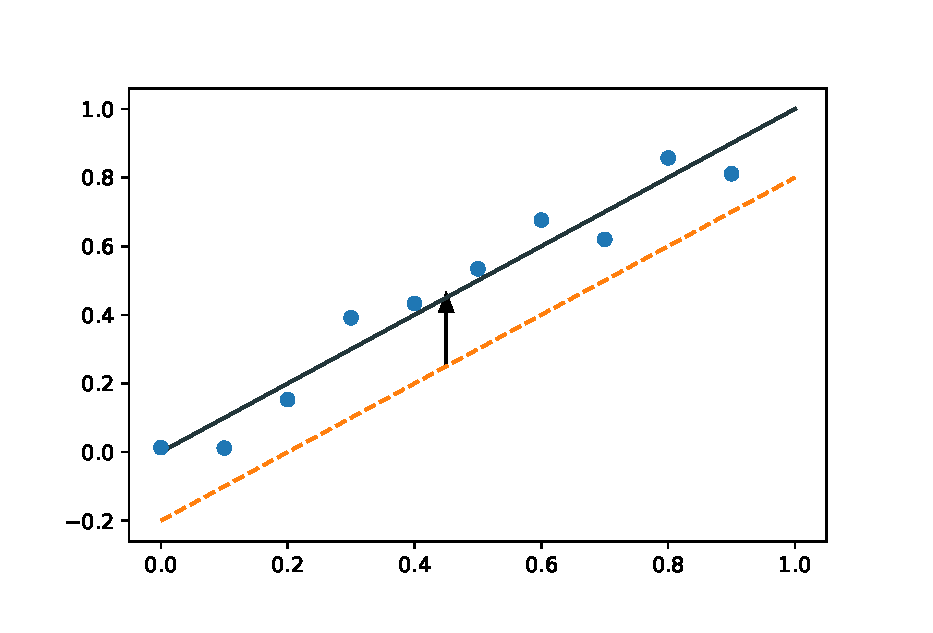
\includegraphics[width=5cm]{fig/arrange_params.eps}
      \caption{{\mgfamily 一次関数のモデルのパラメタ調整}}
    \end{figure}
  \end{columns}
\end{frame}
\section{Classification}
\begin{frame}{{\mgfamily 分類}}
  クラスに分類された既存データを元に新規データを分類する

  \vspace{20pt}
  アルゴリズム
  \begin{itemize}
  \item パーセプトロン
  \item ロジスティック回帰
  \end{itemize}
%  \begin{table}
%    \caption{{\mgfamily アルゴリズムとパラメタの決め方}}
%    \begin{tabular}{@{} ll @{}}      
%      \toprule
%      アルゴリズム &パラメタの決め方\\
%      \midrule
%      パーセプトロン & 確率的勾配降下法\\
%      ロジスティク回帰 & 最尤推定法\\
%      \bottomrule
%    \end{tabular}
%  \end{table}
\end{frame}
\section{Perceptron}
\begin{frame}{{\mgfamily パーセプトロン, モデル}}
  線形なモデル$f$を設定する
  \begin{columns}[T,onlytextwidth]
    \column{0.50\textwidth}
    \[f(x,y)=w_0+w_1x+w_2y\]
    \[f(x,y)>0\Rightarrow t = +1\]
    \[f(x,y)<0\Rightarrow t = -1\]
    \column{0.50\textwidth}
    \begin{figure}
      \centering
      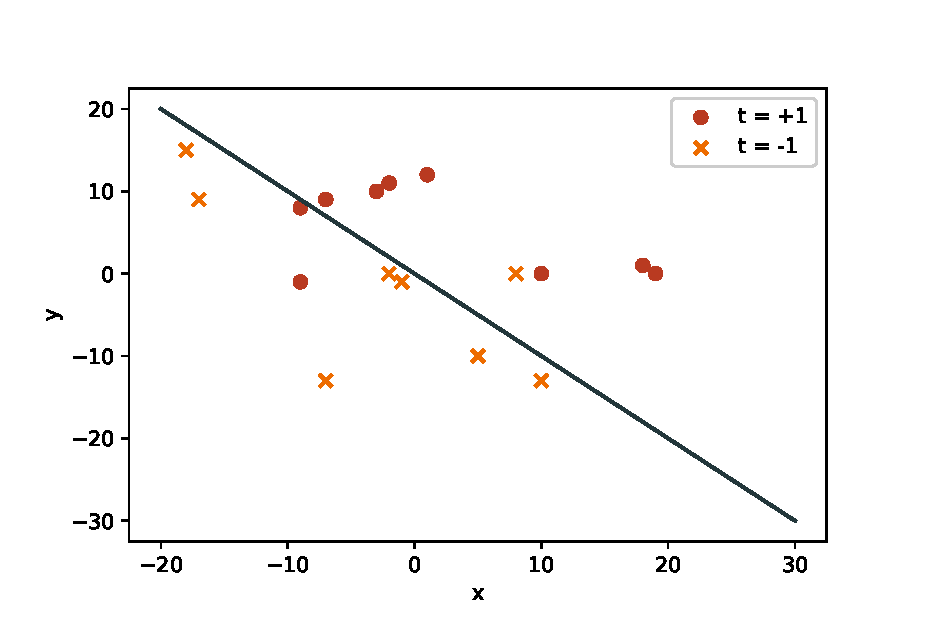
\includegraphics[width=5cm]{fig/scatter.eps}
      \caption{{\mgfamily 属性値$t=\pm1$をもつデータ群}}
    \end{figure}
  \end{columns}
  直線上の点$(x',y')$は$f(x',y')=0$をみたす
\end{frame}
\begin{frame}{{\mgfamily パーセプトロン, 評価基準(誤差関数)}}
  誤差関数$E$が最小になる$w_i$を求める
  \begin{columns}[T,onlytextwidth]
    \column{0.50\textwidth}
    \begin{align*}
      E
      &=\sum_{i=1}^{N}{\left\{-\left(w_0+w_1x+w_2y\right)t_i\right\}}\\
      &=\sum_{i=1}^{N}{\left(-f(x_i,y_i)t_i\right)}
    \end{align*}
    \begin{itemize}
    \item $N$はデータ数
    \item 誤分類だと$-f(x_i,y_i)t_i>0$
    \end{itemize}
    \column{0.50\textwidth}
    \begin{figure}
      \centering
      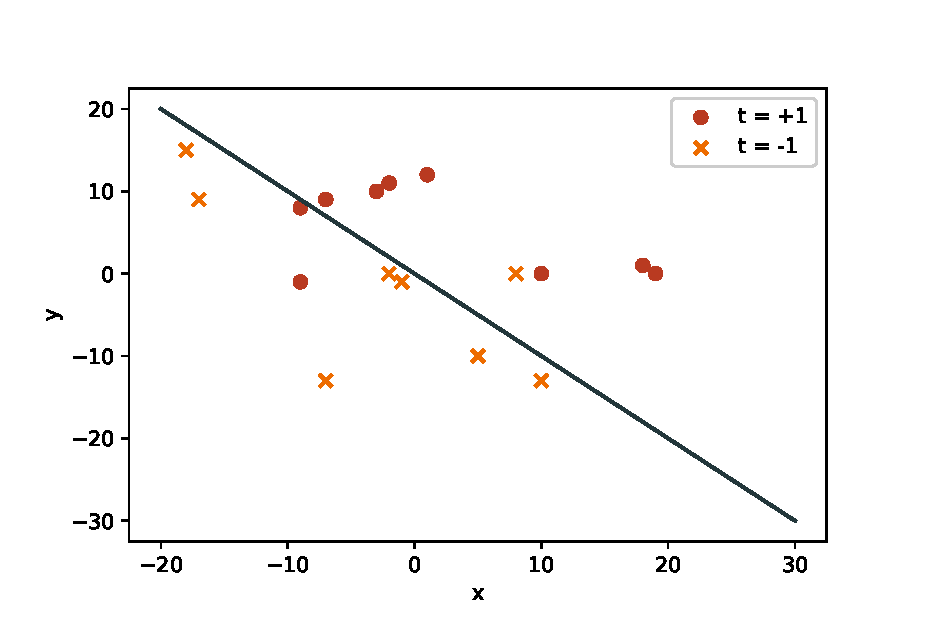
\includegraphics[width=5cm]{fig/scatter.eps}
      \caption{{\mgfamily 属性値$t=\pm1$をもつデータ群}}
    \end{figure}
  \end{columns}
\end{frame}
\begin{frame}{{\mgfamily ロジスティック回帰, モデル}}
  パーセプトロンと同じく線形モデル$f$を設定する
  \begin{columns}[T,onlytextwidth]
    \column{0.50\textwidth}
    \[f(x,y)=w_0+w_1x+w_2y\]
    \[f(x,y)>0\Rightarrow t = +1\]
    \[f(x,y)<0\Rightarrow t = -1\]
    \column{0.50\textwidth}
    \begin{figure}
      \centering
      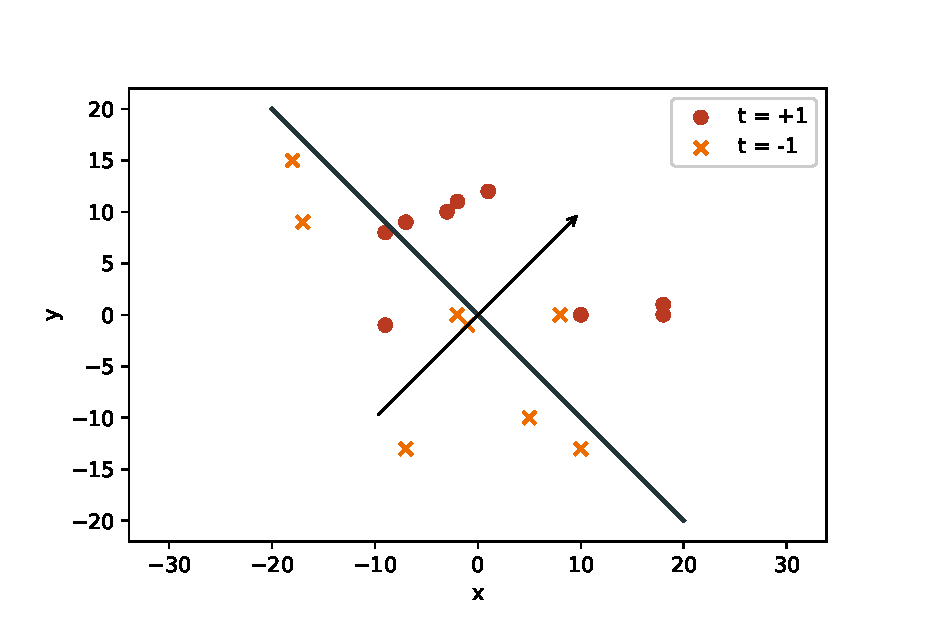
\includegraphics[width=5cm]{fig/direction.eps}
      \caption{$f(x,y)${\mgfamily が増加する向き}}
    \end{figure}
  \end{columns}
\end{frame}
\begin{frame}{{\mgfamily ロジスティック回帰, モデル}}
  ただし,$|f|$が大きいほど$t$である確率が高いとする
  \begin{columns}[T,onlytextwidth]
    \column{0.50\textwidth}
    ロジスティック関数
    \[\sigma\left(\alpha\right)=\frac{1}{1+e^{-\alpha}}\]
    を導入し,\\
    $(x',y')$が$t=1$である確率を\\
    \[0 < \sigma \left(f\left(x',y'\right)\right) < 1\]
    とする
    \column{0.50\textwidth}
    \begin{figure}
      \centering
      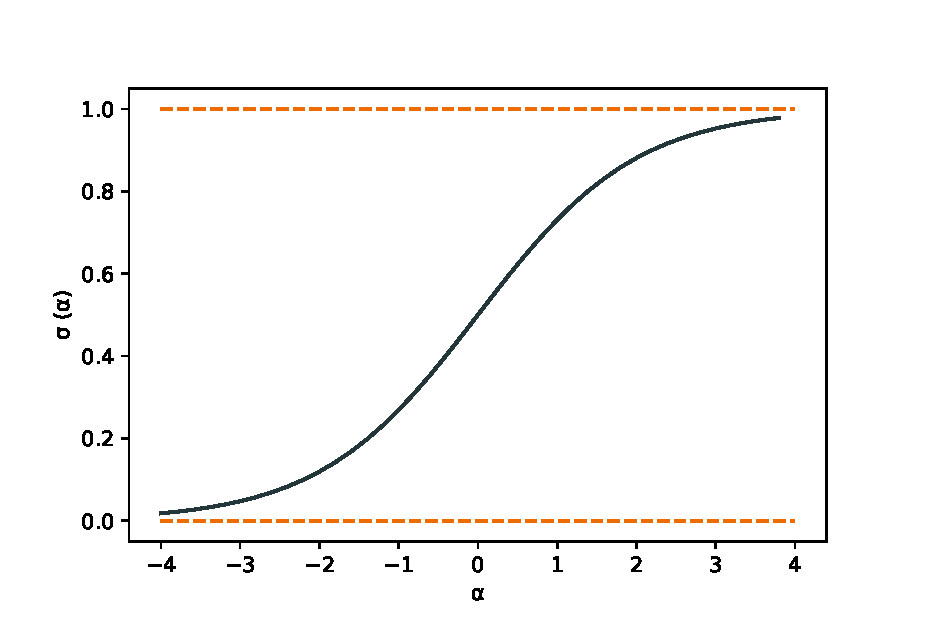
\includegraphics[width=5cm]{fig/sigmoid.eps}
      \caption{{\mgfamily ロジスティック関数のグラフ}}
    \end{figure}
  \end{columns}
\end{frame}
\begin{frame}{{\mgfamily ロジスティック回帰, 評価基準(最尤推定)}}
  訓練データが得られる確率$P$を最大にする$w_i$を求める

  \begin{align*}
    p(x,y)&=\sigma(x_0+w_1x+w_2y)\\
    P&=\prod_{i}^{N}{p\left(x_i,y_i\right)}^{t_n}{\left\{1-p\left(x_i,y_i\right)\right\}}^{1-t_n}
  \end{align*}  
  訓練データは最も発生確率が高いデータであると仮定している
\end{frame}
\section{Regression}
\begin{frame}{{\mgfamily 回帰分析, モデルと評価基準(最小二乗)}}
  データが$M$次多項式$f$に従うとして,二乗誤差$E_D$を最小にするパラメタ$w_{\textit{i}}$を選ぶ
  \begin{columns}[T,onlytextwidth]
    \column{0.50\textwidth}
    \begin{align*}
      f(x)&=\sum_{m=0}^{M}w_mx^{m}\\
      E_{D}&=\frac{1}{2}\sum_{n=1}^{N}{\left\{f(x_n)-t_n\right\}}^2
    \end{align*}
    \column{0.50\textwidth}
    \begin{figure}
      \centering
      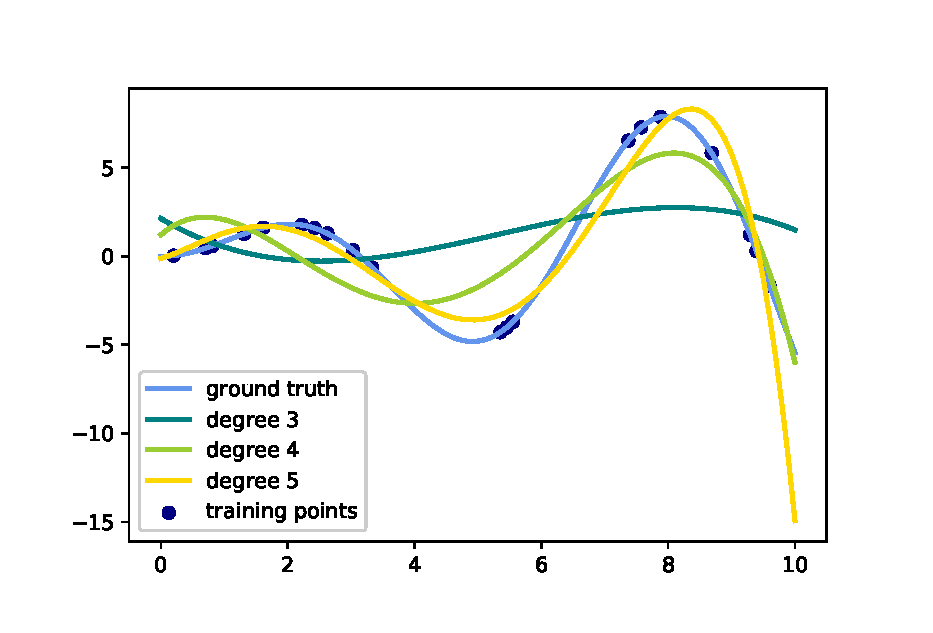
\includegraphics[width=5cm]{fig/polyreg.eps}
      \caption{$M\in\{3,4,5\}${\mgfamily の多項式近似例}}
    \end{figure}
  \end{columns}
\end{frame}
\part{Unsupervised Learning}
\section{Clustering}
\begin{frame}{{\mgfamily k平均法}}
  データ間の距離を求め,データをk個のクラスタに分ける
  \begin{columns}[T,onlytextwidth]
    \column{0.50\textwidth}
    \begin{figure}
      \centering
      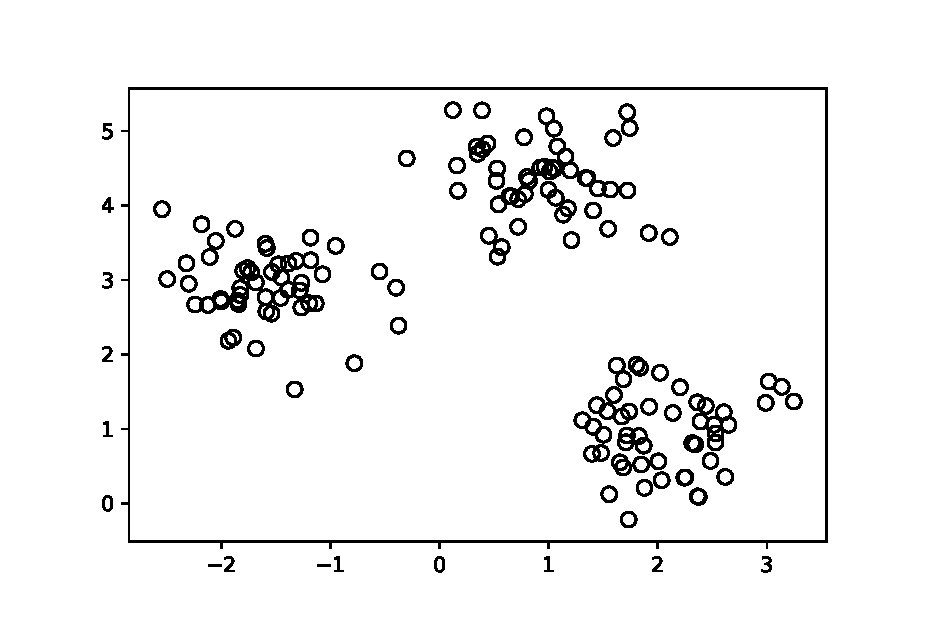
\includegraphics[width=5cm]{fig/cluster.eps}
      \caption{{\mgfamily データ集合}}
    \end{figure}
    \column{0.50\textwidth}
    \begin{figure}
      \centering
      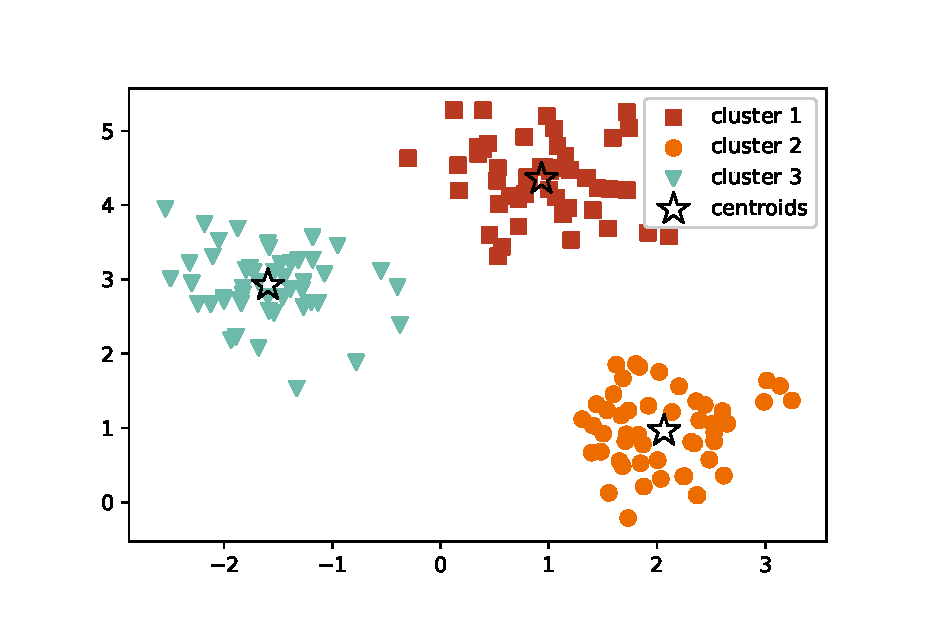
\includegraphics[width=5cm]{fig/colored_scatter.eps}
      \caption{$k=3${\mgfamily のクラスタ}}
    \end{figure}
  \end{columns}
  クラスタごとに代表データを決め,代表の近くのデータ集合で\\クラスタを作る
\end{frame}
\begin{frame}{{\mgfamily k平均法のアルゴリズム}}
  \begin{align*}
    \text{入力}&\text{: データ集合}D=\left\{\mathbf{x}^{(1)},\mathbf{x}^{(2)},\cdots,\mathbf{x}^{(|D|)} \right\}\\
   &\text{: クラスタ数}k
  \end{align*}  
  無作為に$\mathbf{m_1}, \mathbf{m_2}\cdots,\mathbf{m_{\textit{k}}}$を決める\\
\texttt{until} 収束\\
\texttt{\ \ foreach} $\mathbf{x^{(\textit{i})}}\in D$\\
\textbf{\ \ \ \ \ \ }$\textrm{c}_{\textrm{max}} = \argmax_{\textrm{c}} \textit{\textrm{sim}}\left(\mathbf{x}^{(\textit{i})},\textbf{m}_{\textit{c}}\right)$ データ集合の分割\\
\textbf{\ \ \ \ \ \ }$\texttt{insert}\ \mathbf{x}^{(\textit{i})}\texttt{into}\ \textrm{c}_{\textrm{max}}$\\
\texttt{\ \ end\ foreach}
\[
\forall \textit{c}, \mathbf{m}_{\textit{c}}=\frac{1}{|\textit{c}|}\sum_{\textit{x}^{(i)}\in \textit{c}}\mathbf{x}^{(\textit{i})}\ \ \text{代表ベクトルを再計算}
\]
\texttt{end until}
\end{frame}
\begin{frame}{{\mgfamily k平均法の適用例}}
  ピクセルの色を似ている代表色に置き換えて減色する
    \begin{columns}[T,onlytextwidth]
    \column{0.50\textwidth}
    \begin{figure}
      \centering
      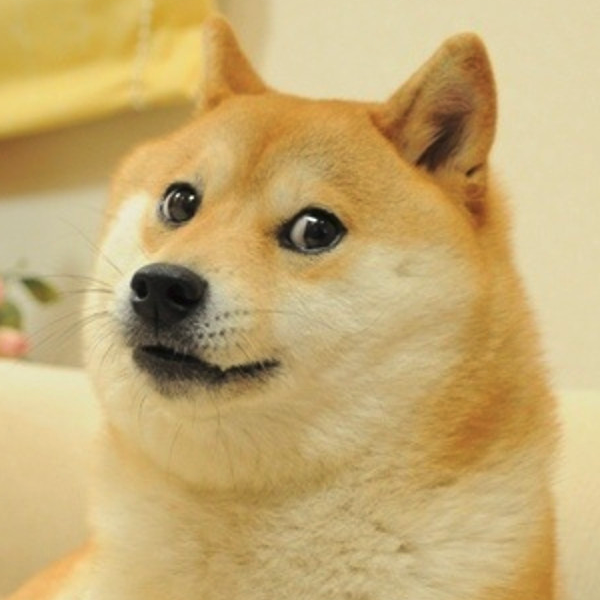
\includegraphics[width=5cm]{fig/doge.png}
      \caption{{\mgfamily 減色前の犬}}
    \end{figure}
    \column{0.50\textwidth}
    \begin{figure}
      \centering
      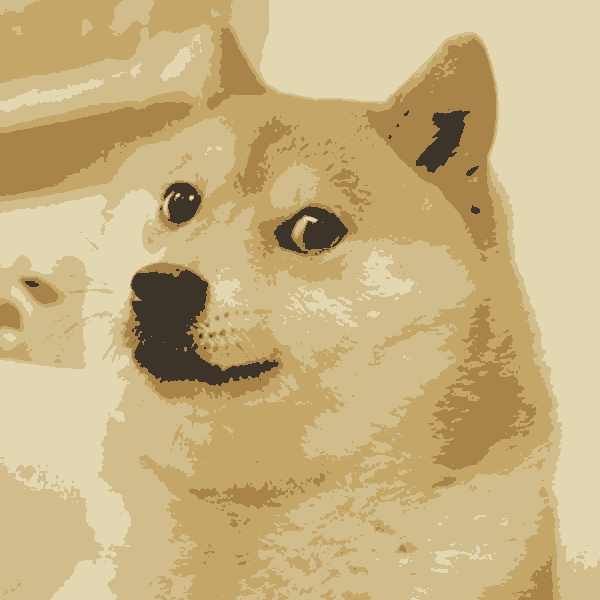
\includegraphics[width=5cm]{fig/doge_q.png}
      \caption{$k=5${\mgfamily で減色された犬}}
    \end{figure}
  \end{columns}
\end{frame}

\end{document}

\begin{frame}{回帰分析, モデル}
  データが$M$次多項式$f$に従うとする
\end{frame}
\begin{frame}{回帰分析, モデル}
  ただし,$x_n$の観測値$t$は正規分布に従い$f(x_n)\pm\sigma$に散らばる  
\end{frame}
\begin{frame}{回帰分析, 評価基準}
  訓練データの集合が生じる確率$P$を最大にするパラメタを求める
\end{frame}
